% Drawing 154/08-1 -- folder 154, batch 08, archive page 141 (PDF page 142).
% Transcription: page de dessins au crayon et à l'encre : deux fuseaux allongés (bigones) traversés de pseudo-droites, l'un en haut à gauche, l'autre en bas à droite ; au milieu, une longue droite marquée $D$ et $D'$ (plusieurs fois), coupée de croisements, un chemin brisé en zigzag qui la longe, des hachures le long de la droite ; à gauche, un disque traversé d'arcs qui se croisent (une sorte de fuseau à sommets marqués) et un grand disque traversé de pseudo-droites ; en haut à droite, des arrangements de droites au crayon ; un rectangle au crayon
% Kind: page of pencil and ink drawings: spindles, a long line D/D' cut by crossings with a broken path, disks. Method 2 (schematic redraw from the facsimile). Status: partial.
% Notes: Page of pencil and ink drawings over a plotter job sheet (25 Aug 82; not reproduced), read from the page view: two elongated spindles (bigons) crossed by pseudolines, top left and bottom right; in the middle a long line marked D and D' (several times) cut by crossings, a broken path in ink along it; disks with arrangements (left); a rectangle; many further pencil lines (only the main ones drawn). The pencilled legends « p.r. stable / sous-stable / critiques » and the formula at the foot are text of the transcription. Still differs from the facsimile: Page of pencil and ink drawings over a plotter job sheet (25 Aug 82; not reproduced), read from the page view: two elongated spindles (bigons) crossed by pseudolines, top left and bottom right; in the middle a long line marked D and D' (several times) cut by crossings, a broken path in ink along it; disks with arrangements (left); a rectangle; many further pencil lines (only the main ones drawn).
% Coordinates: 1 unit = 1 mm = 1/100 of the crop width (bbox in page fractions: [0.139, 0.124, 0.964, 0.496]).
% Redrawn by Claude (claude-opus-5-5), issue #73, 2026-11-07; not checked by a human; not compiled (no TeX in the session).
% Revised by Claude (claude-opus-5-5) 2026-11-09 (issue #128) after Michel's check: vertices snapped to exact intersections (drawn points on their lines, meeting ends on the stroke they meet, near-concurrent lines through one computed point, curve ends on their rim); labels at \small as in folder 80 batch 3. Status: partial.
% Rights: reproduces part of the work -- behind RENDER_TRANSCRIPTS, never published by itself.
\documentclass[tikz,border=3pt]{standalone}
\usepackage{amsmath,amssymb}
\usetikzlibrary{patterns,arrows.meta}
\tikzset{Or/.style={orange!90!black}, Ye/.style={yellow!80!orange}, Lg/.style={green!60!black!70}, Dg/.style={green!45!black}, Br/.style={brown!80!black}, Rd/.style={red!85!black}, Bl/.style={blue!70!black}, Gy/.style={black!40}, pencil/.style={black!45}, struck/.style={black!35}, mark/.style={circle,draw,inner sep=1.3pt}, pt/.style={circle,fill,inner sep=0.9pt}, opt/.style={circle,draw,fill=white,inner sep=1.1pt}}
\begin{document}
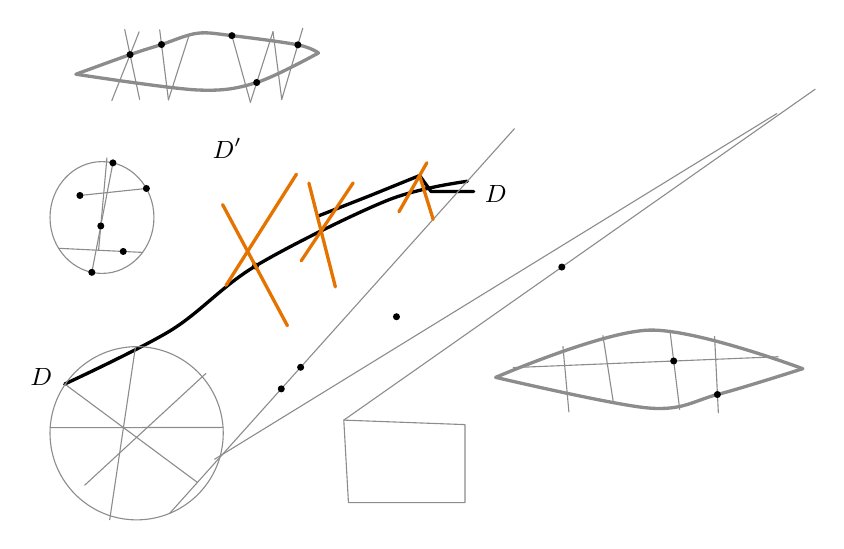
\begin{tikzpicture}[x=1mm,y=1mm,line cap=round,line join=round,font=\scriptsize]
\draw[pencil,very thick] plot[smooth, tension=0.55] coordinates {(4.4,-7.1) (11.27,-4.61) (15.26,-3.33) (19.8,-1.9) (24.2,-2.2) (32.58,-3.37) (35.2,-4.4)};
\draw[pencil,very thick] plot[smooth, tension=0.55] coordinates {(4.4,-7.1) (19.8,-9.1) (27.35,-8.15) (35.2,-4.4)};
\draw[pencil] (10.59,-1.43) -- (12.48,-10.3);
\draw[pencil] (15.03,-1.46) -- (16.14,-10.36);
\draw[pencil] (24.2,-2.2) -- (26.55,-10.66);
\draw[pencil] (29.42,-1.7) -- (30.53,-10.3);
\draw[pencil] (12.42,-1.72) -- (8.95,-10.45);
\draw[pencil] (18.79,-2.06) -- (16.14,-10.36);
\draw[pencil] (29.42,-1.7) -- (26.55,-10.66);
\draw[pencil] (33.2,-1.26) -- (30.53,-10.3);
\node[pt] at (11.27,-4.61) {};
\node[pt] at (15.26,-3.33) {};
\node[pt] at (24.2,-2.2) {};
\node[pt] at (27.35,-8.15) {};
\node[pt] at (32.58,-3.37) {};
\draw[very thick] plot[smooth, tension=0.55] coordinates {(2.97,-46.45) (16.5,-39.6) (27.19,-31.46) (44,-23.1) (54.1,-20.7)};
\draw[very thick] (35.05,-25.15) -- (41.8,-22.5) -- (48.03,-19.97) -- (49.5,-22) -- (54.9,-22);
\node[inner sep=1pt] at (57.7,-22.3) {\small $D$};
\node[inner sep=1pt] at (23.6,-16.5) {\small $D'$};
\node[inner sep=1pt] at (0,-45.6) {\small $D$};
\draw[pencil] (16.31,-62.86) -- (60.08,-14.02);
\draw[pencil] (22,-56) -- (93.4,-12.1);
\draw[pencil] (38.41,-51.03) -- (98.27,-9.01);
\node[pt] at (27.19,-31.46) {};
\node[pt] at (45.1,-37.9) {};
\node[pt] at (66.1,-31.59) {};
\node[pt] at (32.93,-44.32) {};
\node[pt] at (30.47,-47.06) {};
\draw[Or,very thick] (23.02,-23.66) -- (31.25,-39.04);
\draw[Or,very thick] (32.4,-19.8) -- (23.46,-33.92);
\draw[Or,very thick] (33.98,-20.93) -- (37.34,-34.11);
\draw[Or,very thick] (39.6,-20.9) -- (33,-30.8);
\draw[Or,very thick] (48.03,-19.97) -- (49.76,-25.53);
\draw[Or,very thick] (48.96,-18.35) -- (45.41,-24.58);
\draw[pencil] (7.7,-25.3) ellipse[x radius=6.6, y radius=7.1];
\draw[pencil] (4.9,-22.5) -- (13.34,-21.61);
\draw[pencil] (7.27,-29.46) -- (8.33,-17.72);
\draw[pencil] (9.09,-18.36) -- (6.41,-32.26);
\draw[pencil] (2.19,-29.21) -- (12.86,-29.73);
\node[pt] at (9.09,-18.36) {};
\node[pt] at (4.9,-22.5) {};
\node[pt] at (13.34,-21.61) {};
\node[pt] at (7.55,-26.37) {};
\node[pt] at (6.41,-32.26) {};
\node[pt] at (10.4,-29.61) {};
\draw[pencil] (12.1,-52.7) circle[radius=11];
\draw[pencil] (2.97,-46.45) -- (19.82,-58.94);
\draw[pencil] (5.5,-59.3) -- (20.9,-45.1);
\draw[pencil] (11.96,-41.7) -- (8.68,-63.68);
\draw[pencil] (1.12,-51.99) -- (23.07,-51.96);
\draw[pencil] (38.41,-51.03) -- (53.8,-51.6) -- (53.8,-61.5) -- (39,-61.5) -- cycle;
\draw[pencil,very thick] plot[smooth, tension=0.55] coordinates {(57.7,-45.6) (77.2,-39.6) (96.7,-44.5)};
\draw[pencil,very thick] plot[smooth, tension=0.55] coordinates {(57.7,-45.6) (77.2,-49.5) (85.86,-47.78) (96.7,-44.5)};
\draw[pencil] (66.24,-41.67) -- (67,-50);
\draw[pencil] (71.32,-40.3) -- (72.67,-48.94);
\draw[pencil] (79.83,-39.64) -- (81.07,-49.67);
\draw[pencil] (85.5,-40.39) -- (85.98,-50.1);
\draw[pencil] (59.93,-44.36) -- (93.57,-42.98);
\node[pt] at (80.31,-43.52) {};
\node[pt] at (85.86,-47.78) {};
\end{tikzpicture}
\end{document}
